\documentclass[conference]{IEEEtran}
% If the IEEEtran.cls has not been installed into the LaTeX system files,
% manually specify the path to it. e.g.
% \documentclass[conference]{./IEEEtran}

% Add and required packages here
\usepackage{graphicx,times,amsmath,fontenc}
\usepackage[hyphens]{url}
% \usepackage{hyperref}

% Correct bad hyphenation here
\hyphenation{op-tical net-works semi-conduc-tor IEEEtran}

% To create the author's affliation portion using \thanks
\IEEEoverridecommandlockouts

\textwidth 178mm
\textheight 240mm
\oddsidemargin -6mm
\evensidemargin -6mm
\topmargin -6mm
\columnsep 5mm

\begin{document}

% Paper title: keep the \ \\ \LARGE\bf in it to leave enough margin.
\title{\ \\ \LARGE\bf Developing Game Strategy for
Monopoly\textsuperscript{\textregistered} \\ Using Genetic Algorithms \thanks{K.
Mukhar is a Master�s Degree candidate at the University of Colorado Colorado
Springs, CO 80918 USA (phone: 1-408-475-6854; e-mail: {\tt kmukhar@uccs.edu}).
J. K. Kalita is with the Department of Computer Science, University of Colorado
Colorado Springs, CO 80918 USA. (e-mail: {\tt jkalita@uccs.edu}). Monopoly is a
registered trademark of Hasbro, Inc. }}

\author{K Mukhar, J K Kalita}

% Uncomment out the following line for invited papers
% \specialpapernotice{(Invited Paper)}

% Make the title area
\maketitle

\begin{abstract}
Games are a rich field of study for artificial intelligence and evolutionary
computation. A great deal of research has been conducted into using AI to solve
deterministic games with complete information. However, research in
non-deterministic games is more limited. This paper details study of the use of
genetic algorithm techniques to evolve game strategies for the multi-player
non-deterministic game Monopoly\textsuperscript{\textregistered}. Populations of
Monopoly\textsuperscript{\textregistered} players were evolved using various
chromosomes and fitness functions. The results showed that it was indeed
possible to evolve players despite the high level of non-determinism and that
the strategies that evolved tracked closely with heuristic rules used by
real-world players.
\end{abstract}

% No keywords

\section{Introduction}
% No \PARstart
In \emph{Theory of Games and Economic Behavior} by Von Neumann and Morgenstern,
games were used to model economics and economic
behavior~\cite{neumann2007theory}. Early work by mathematicians studying card
and dice games led to the development of statistics and
probability~\cite{hald1990history,rudas2008handbook}. Games can be used to study
how social behavior and human interactions affect and are affected by game
play~\cite{fararo1992meaning}. A great deal of artificial intelligence research
deals with developing AI game players and finding optimum game
strategies~\cite{russell2010artificial}.

Early research into AI and games tended to focus on developing algorithms for
searching the space of legal moves. This research led to such techniques as the
Min-Max algorithm~\cite{neumann2007theory} and the A* search
algorithm~\cite{Hart_Nilsson_Raphael_1968,Flood1958}.

Researchers have used genetic algorithms and evolutionary computation to
investigate whether optimal strategies for games can be evolved. Much of that
research has focused on two player deterministic games like The Prisoner's
Dilemma and Tic-Tac-Toe. Evolutionary computation techniques have been used with
good success for these types of
problems~\cite{Nowak1993,DBLP:conf/cig/QuekG07,Fogel1993}.

However, there are other classes of games such as multi-player non-deterministic
games where the search space is potentially quite large and the cost function
could have multiple local and global optima. Evolutionary computation could be
an effective approach to these types of problems because it provides the
capability to traverse a large search space and find optimal strategies.

This study investigates using evolutionary computation to evolve game strategies
for these types of games. In general, this study evaluated whether genetic
algorithms can be used to develop strategies for non-deterministic games.
Specifically, genetic algorithms were applied to the non-deterministic game
known as Monopoly\textsuperscript{\textregistered} to evolve game playing strategies.

The rest of this paper is organized as follows. Section II reviews related
research in applying genetic algorithms to various games from the relatively
simple Prisoner�s Dilemma to more complicated games such as Othello. Section III
presents a discussion of the game of Monopoly\textsuperscript{\textregistered},
focusing on the rules of the game and various heuristic strategies that have
been developed since the game�s introduction. Based on the rules and heuristics,
a genetic algorithm is designed and presented in Section IV. Section V presents
the results of evolving a population of
Monopoly\textsuperscript{\textregistered} players, using various fitness
functions. Finally, Section VI summarizes the results and discusses future
research directions.

\section{Background}

Holland, in his seminal work \emph{Adaptation in Natural and Artificial
Systems}, discussed applications of genetic algorithms to games~\cite{Holland1992}.
Holland showed that the search space of many games quickly grew to a size that
is not computationally tractable. He discussed how an artificial adaptive system
(i.e., evolutionary computation) could be used to efficiently search the game
space and realize an optimal strategy. Some of the research that applied
Holland�s ideas to the study of games is summarized below.

\subsection{Deterministic zero sum games}

One of the most studied games is the two person game known as the Prisoner's
Dilemma, a game in which two players can either cooperate or defect, without the
ability to communicate with each other. In a single iteration of this game, the
best strategy for both players is to defect~\cite{nash50,Nash1951}. However,
studies have shown that when the game is played repeatedly between two or more
players (known as the Iterated Prisoner's Dilemma game), a strategy of
cooperation will evolve
spontaneously~\cite{Nowak1993,DBLP:conf/cig/QuekG07,Axelrod5,mittal2009,wang5573053}.

The game of Tic-Tac-Toe is a relatively simple two-player competitive game
played on a 3x3 grid. Players alternately place a symbol, (usually one player
plays X and the other plays O) on an open grid space; the winner is the player
that manages to create a straight line (vertically, horizontally, or diagonally)
of three of his own symbols. Fogel showed that genetic algorithms could be used
to evolve neural networks to play the game~\cite{Fogel1993}. The game also can
be solved using a pure genetic algorithm, with the genome encoding the different
game board permutations.

In Checkers each player has 12 pieces that can move diagonally on a board
divided into an 8x8 grid of squares. If one player's piece is adjacent to the
opponent's piece, and there is a blank square on the opposite side of the
opponent's piece, the player can jump that piece and remove the opponent's piece
from the board. The winner is the player who removes all of the opponent's
pieces from the board. Fogel and Chellapilla used a neural network that was
optimized using evolutionary computing and then tested the network in an on-line
tournament. Their evolved ANN player was able to play at Expert
level~\cite{Fogel2000Anaconda,journals/tec/ChellapillaF01}.

Othello (also known as Reversi) is a two-player game where players take turns
placing colored tokens on the board. The winner is the player who can get the
most tokens of his color on the board. Play is complicated by the fact that a
player can only place a token in a way that ``captures'' the opponent's tokens.
This is done by placing a token adjacent to an opponent's token such that at
least one of the opponent's tokens lies between the new token and one of the
already placed tokens. When a player captures a line of the opponent's tokens,
all of the opponent's tokens in that line change to the capturing player's
color. Chong, et al., investigated evolving the evaluation function of a neural
network to create an ANN that could play Othello~\cite{ChongTW05}.

Even for games of much higher complexity, genetic algorithms have been used with
success. Genetic algorithms have been applied to games such as
Chess~\cite{Mitsuta:2010:OPG:1994486.1994517} and
Go~\cite{shah2012Go,Blackman2009Go}.

These deterministic, two-player, zero-sum games are widely studied because
they are relatively simple to understand and play. Most of them have a relatively
limited search space (Othello, Chess and Go being obvious exceptions), which
makes them tractable to study and simulation. However, there is a whole class of
games, with many examples that are non-deterministic, multi-player (but still
usually zero-sum) games. While not as well studied as the two player games
mentioned previously, there has been some research on using evolutionary
computation to create winning strategies for these games.

\subsection{Monopoly\textsuperscript{\textregistered} - A Non-Deterministic
game}

Monopoly\textsuperscript{\textregistered} is a game where players traverse a
path around a board on which most spaces represent a property (See
Figure~\ref{figure-fig1}) which players can buy. Other players must pay ``rent''
to the owner of a property when they land on that property.
When one player owns all the properties in a color group (a monopoly), the
player can ``develop'' the properties by building houses or hotels. This
increases the rent value which increases the odds that an opponent will not be
able to pay the rent. If a player cannot pay rent, he must sell or mortgage
properties, and if that is not possible, give their properties to the owner. The
winner is the player who bankrupts the other players. Some of the first studies
of the game were statistical analyses of which properties were more valuable to
own~\cite{Ash1972}. Frayn used evolutionary computing to develop an efficient
strategy for property valuation and property
management~\cite{DBLP:conf/cig/Frayn05}. Another important feature of
Monopoly\textsuperscript{\textregistered} is the ability of players to trade
different properties. Because of the random nature of a player's moves, it is
improbable that a single player will be able to land on and buy all the
properties in a group. So, players usually must trade with other players to gain
a monopoly on a property group. Yasumura, et al., studied different negotiating
strategies to identify the best way to conduct negotiations between
players~\cite{Yasumura2001Negotiate}.

\begin{figure}[htp]
\centerline{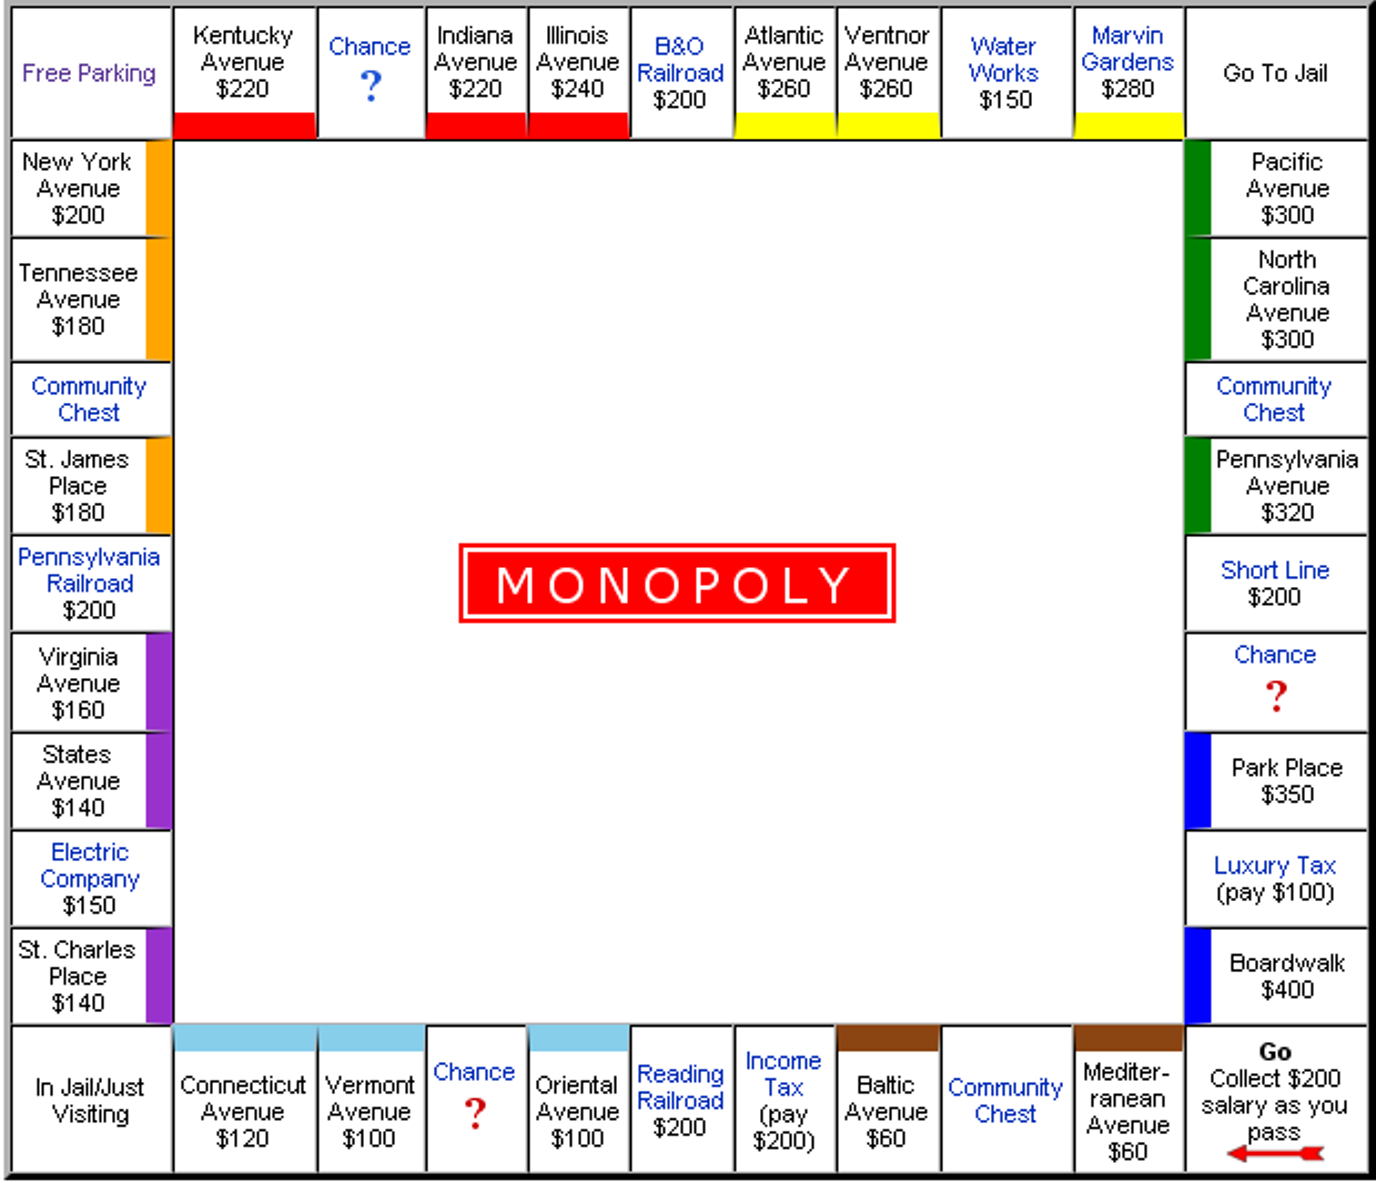
\includegraphics[width=1.0\columnwidth]{Monopoly.png}}
\caption{The board layout for Monopoly. For this study, the edge of the board
containing ``Go'' through ``Connecticut Avenue'' is South. Proceeding clockwise,
the next edge is West. The top of the figure is North. The final edge of the
board is East. South includes the cheapest properties; East contains the most
expensive. Monte Carlo simulations of dice rolls show that the most landed on
locations are on the West and North edges of the board.}
\label{figure-fig1}
\end{figure}

\section{Overview of the Game of Monopoly\textsuperscript{\textregistered}}
\subsection{Rules of Monopoly\textsuperscript{\textregistered}}

Monopoly\textsuperscript{\textregistered} is a board game that consists of a
four-sided game board, with 40 spaces along the sides of the board where a
player can land as they move around the board (See Figure~\ref{figure-fig1}). As
players move around the board, they can buy and sell property using play money.

All the players in the game start with \$1500 at the corner space marked ``GO.''
Each player is represented by a game token on the board. The players take turns
rolling two six-sided dice and moving their game token by as many spaces as the
value of the dice. Thus, for each move, a player will move between 2 and 12
spaces.

If a player rolls doubles the player moves the token, takes any actions
necessary, and then the player is allowed a second roll of the dice. If the
player rolls doubles on the second roll, the player is allowed a third roll. If
the player rolls doubles a third time, they must move their token directly to
the space marked ``Jail.''

There are 28 locations on the game board that can be bought by the players. The
locations are divided into 22 streets grouped into 8 color groups, 4 railroads,
and 2 utilities. If the player lands on an un-owned location, the player may buy
the property. If the player declines to buy the property, the property is
auctioned among all players (including the player who originally declined to buy
the property). If the player lands on a property that is already owned, the
player must pay rent to the owning player.

Once a player obtains all properties within a group, the properties can be
``improved'' by building houses or hotels on the property. Improved properties
have a higher rent.

The other 12 locations on the board cannot be owned by any player. For this
study, only one of those locations is important. That location is the corner
space marked ``Jail.'' There are three circumstances that can send a player to
Jail: drawing a special card marked ``Go To Jail,'' landing on the corner marked
``Go To Jail''; or rolling doubles three times in a row in one turn.

A player whose token is in Jail may, on their next turn, pay \$50, roll the dice,
and leave jail; or the player may choose to attempt to roll doubles to leave
jail. If the player has not rolled doubles on the third attempt, the player must
immediately pay \$50 and move the number of spaces shown on the dice.

The complete set of rules can be accessed at
\url{http://www.hasbro.com/common/instruct/monins.pdf}.

\subsection{Game Strategies}

In the past, the official web site for the game provided a list of useful game
strategies. (accessible at
\url{http://web.archive.org/web/20080516095129/http://www.hasbro.com/games/kid-games/monopoly/default.cfm?page=StrategyGuide/play_to_win}).
Some of those strategies are as follows.

\begin{enumerate}

\item Buy a property if no other player owns a property in its color group.

\item Buy a property if it gives you a second or third property of its group.

\item Buy a property if it blocks an opponent from controlling a color group.

\item Buy a property if it is an orange property (always block this group if you
can).

\item Pay \$50 and get out of Jail early in the game while many
Monopoly\textsuperscript{\textregistered} properties remain un-owned and
undeveloped.

\item When most Monopoly\textsuperscript{\textregistered} properties are
developed between Jail and the Go to Jail space, roll the dice and hope to stay
in Jail.

\end{enumerate}

\section{Methodology}

A survey of previous research found only two computer science papers: the
previously cited study by Frayn~\cite{DBLP:conf/cig/Frayn05} of using
evolutionary computing to evolve property evaluations, and the study by
Yasumura, et al., of negotiating strategies~\cite{Yasumura2001Negotiate}. In
addition, there have been analytical studies and Monte Carlo simulations of the
statistics and probability of landing on any particular location in
Monopoly\textsuperscript{\textregistered}~\cite{Ash1972,Abbot1997}.

A finite state machine was used to model player actions. In many cases, the
transition from state to state is made automatically without input from the
player. For example, a player always has to roll the dice to move around the
board; this event does not require any input or decision from the player.
However, analysis of the state machine revealed four state transitions that do
require a decision on the part of the player.

\begin{enumerate}

\item The player must decide whether or not to buy a property. If a property is
being auctioned, the player must decide whether and how much to bid for the
property.

\item The player must decide whether to pay bail and exit jail immediately, or
roll the dice and wait until doubles are rolled.

\item The player must decide when and how to buy houses or hotels for their
properties.

\item The player must decide if and when to trade for properties to complete a
monopoly.

\end{enumerate}

Based on the rules of Monopoly\textsuperscript{\textregistered} and previous
analytic studies, the following focus areas were enumerated.

\begin{enumerate}

\item Decisions on whether to buy a property depend on what other properties
have been acquired and which players have acquired them.

\item The decision of whether to stay in jail or leave jail depends on what
other properties have been acquired and which players have acquired them.

\item There are a limited number of buildings in the game. Whether one can build
depends on what other players have built, and vice versa.

\item The ability to develop a property group depends on the ability of the
player to acquire all the properties in a group. This is done by trading with
other players.

\end{enumerate}

These focus areas resulted in a preliminary decision to use a multiple
chromosome strategy in which different chromosomes control the player behavior
depending on the state of the game: one strategy for early in the game when few
properties are owned; a different strategy for later in the game when many
properties are owned. Frayn used a similar strategy, except in his study, the
valuation of a property depended on ownership and development factors and the
genome used that valuation to make decisions.
 
Additionally, this study focused on just two decisions that the player would
make: the buy property decision (item 1 from the list above) and the get out of
jail decision (item 2). The other two decisions, whether to build a house (item
3) and whether to trade a property (item 4), were not implemented using genetic
computation. The house building decision was implemented as a rule based
algorithm; the property trading decision was not implemented.

\subsection{Chromosome Description}

The genome for the evolved player consists of multiple chromosomes; each
chromosome is used for a different purpose or state of the game. This is in
contrast to the classic simple GA where each member of the population has a
single chromosome that is expressed as a string of binary digits. Following the
initial description of the primary chromosome used in this study, two alternate
versions of the chromosome will be described.

The first set of chromosomes consists of 4 arrays of doubles, 40 elements per
array (See Table~\ref{table-chromo}). In this paper, this chromosome is referred
to as the RGA Player (RGA for Real-valued Genetic Algorithm). Each element of the array
represents the probability that the player will purchase the property
represented by the array element. There are 40 locations on the
Monopoly\textsuperscript{\textregistered} board, so each location corresponds
to an element in the array. The �Go� space is element 0, with subsequent
locations assigned successive element indices. However, only 28 locations can be
owned by a player, so 12 of the array elements are ignored. The chromosome could
have contained only 28 locations, but by using 40 elements, the need to create a
mapping between locations and array elements is avoided (for improved code
readability and maintainability) at a small cost of memory for the 12 unused
elements. Each array corresponds to one of the following game states.

\begin{enumerate}

\item The first array is used when no player owns any property in the group
where the player is currently located.

\item The second array is used when the current player owns at least one
property in the group where the player is currently located and no other player
owns property in that group.

\item The third array is used when one other player owns property in the
property group where the player is currently located.

\item The fourth array is used when two other players both own property in the
property group where the player is currently located. Based on the game
strategies listed earlier the 4th chromosome will tend to have values that are
generally less than the values in the 1st, 2nd and 3rd chromosomes. That is, the
player should be more likely to buy property when no other player owns any
properties in the group (1st chromosome), when the property is needed to
complete a monopoly (2nd chromosome), and when the property is needed to block
another player (3rd chromosome).

\end{enumerate}

\begin{table}[h]
\caption{Chromosome Illustration}
\begin{center}
\begin{tabular}{|l|c|c|c|c|}
\hline
\multicolumn{1}{|l|}{\raisebox{-1.50ex}[0cm][0cm]{Location\!}}
& \multicolumn{1}{|c|}{Chr1}
& \multicolumn{1}{|c|}{Chr2}
& \multicolumn{1}{|c|}{Chr3}
& \multicolumn{1}{|c|}{Chr4} \\ \hline
0 - Go &  ignored  &  ignored &  ignored & ignored \\ \hline 
1 - Mediterranean Ave &  $0.615$  &  $0.540$  &  $0.611$ & $0.654$ \\ \hline 
2 - Community Chest &  ignored  &  ignored &  ignored & ignored \\ \hline
3 - Baltic Ave &  $0.288$  &  $0.532$  &  $0.165$ & $0.088$ \\ \hline
4 - Income Tax &  ignored  &  ignored &  ignored & ignored \\ \hline
5 - Reading Railroad & $0.129$  &  $0.649$  &  $0.965$ & $0.390$ \\ \hline
6 - Oriental Ave & $0.834$  &  $0.310$  &  $0.593$ & $0.738$ \\ \hline
Etc\ldots & & & & \\ \hline
\end{tabular}
\label{table-chromo}
\end{center}
\end{table}

The other set of chromosomes is used to determine when to pay to get out of
jail, and when to remain in jail (and hopefully not roll doubles with the dice).
This chromosome is a 2-D array of doubles.

Rows and columns in the array are indexed by 6-bit numbers created by the
properties on one side of the board. The first index corresponds to the West
side of the board; the second index corresponds to the North side of the board.
For each property on the West/North side of the board, the corresponding bit in
the index is set to 1 if the property is owned by some other player; otherwise,
it is set to 0. Thus there are two indices with values that range from 0 to 63.

The value at each element of the array is a double which represents the
probability that the player will choose to pay the bail. Note that this scheme
automatically accounts for different game states: early in the game, very few of
the properties are owned (none when the game begins) so the indices will be near
(0, 0); later in the game, if many properties are owned by other players, the
indices will be near (63, 63). It also accounts for differences in ownership.
That is, if opponents own many properties on the West and North edges, the
indices will be relatively high, whereas if the player owns many of the
properties, the indices will be relatively low. So, if the player owns
properties near the jail, his jail decision will be similar to the decision made
early in the game when few properties are owned.

\subsection{Alternate Jail Chromosome}

Because the 64x64 array described above consumes a relatively large amount of
memory, this study also looked at an alternate genome which varied the ``Get Out
Of Jail'' chromosome by making it a 4x4 array. Instead of indexing by which
players owned properties on the West and North edges of the board, the index was
created by determining if any of the four groups are part of a monopoly owned by
an opponent. This only requires a two-bit index and 16 array elements. The
player using this chromosome will be referred to as the TGA Player.

\subsection{Alternate Chromosome Description}

Goldberg described the structure of a simple GA (SGA) in \emph{Genetic
Algorithms in Search, Optimization, and Machine
Learning}~\cite{goldberg1989genetic}. The SGA uses a single string of binary
bits for its chromosome. Although the primary population used in this study
consists of real valued chromosomes described above, the same information could
be encoded into binary strings.

We start by converting each element (gene) in the original chromosome into a 6
bit number. Each element in the original chromosome now has a value that ranges
from 0 to 63, or a coarseness of approximately 1.6\% for each decision. Then we
take all the genes and concatenate them into a single string. So, for example,
the first chromosome of 40 elements becomes a single string of 240 bits (6 bits
* 40 elements). Each of the other property buying chromosomes is encoded in the
same way.

The ``Get Out Of Jail'' chromosome is then encoded as a 96 bit string (16 genes x
6 bits per gene). This chromosome uses the simplified indexing scheme described
previously in Section C.

\subsection{Population Evolution}

Following Frayn~\cite{DBLP:conf/cig/Frayn05}, Table I shows the genetic
algorithm parameters used for creating and evolving the population of game
players.

\subsection{Fitness Evaluation}

Five different fitness evaluations were used for the genetic algorithm. The
winner of each game is the last player left in the game, or the player with the
greatest net worth when the game finishes. The second place player is the second
to last player in the game, or the player with the second greatest net worth
when the game finishes. Third and fourth place players are determined similarly.
The different evaluators awarded points to the players as follows.

\begin{enumerate}

\item Number of wins (NUM\_WINS); the winner of each game receives three points;
all other players receive zero points.

\item Number of Properties owned (NUM\_PROPERTIES); each player receives one
point per property owned at the end of the game.

\item Number of Monopolies (NUM\_MONOPOLIES); each player receives one point for
each monopoly they control.

\item Finish Order (FINISH\_ORDER); in a game with \(n\) players, the winner of
the game receives \(n-1\) points; second place receives \(n-2\) points, and so
on. The last place finisher receives 0 points.

\item Net Worth (NET\_WORTH); at the end of each game, the net worth of each
player is calculated. Each player receives points that equal their net
worth/100.

\end{enumerate}

\subsection{Procedure}

The genetic algorithm proceeds as follows:

\begin{enumerate}

\item Initialize a population of 1000 individuals.

\item At the start of a generation, the 1000 individuals are randomly divided
into 250 sets of 4.

\item These 250 sets each play an individual game. At the conclusion of each
game, the fitness evaluator for that population computes points for the game and
adds the points to the player�s fitness score. After all 250 games are complete,
the 1000 individuals are again randomly divided into 250 different sets, and the
sets play again until each player has played 100 games.

\item At the end of the generation, the total number of points earned by each
individual is evaluated as the fitness of the individual.

\item The new population of 1000 players is created using this procedure:

\begin{enumerate}

\item the top 10\% (approximately 100 players) survive to the next generation;

\item three hundred more (30\%) survive based on a roulette selection with
replacement;

\item three hundred more (30\%) are selected based on a roulette selection with
replacement and then mutated for the next generation;

\item the final 300 individuals are created by selecting parents using roulette
wheel selection, and then combing the chromosomes to create two new children.
For the RGA and TGA players with real-valued chromosomes, the child chromosomes
are created by blending each parent gene using these formulas
from~\cite{adewuya1996new}:

\begin{equation*}
child_1 = \beta parent_1 + (1-\beta)parent_2
\end{equation*}
\begin{equation*}
child_2 = (1-\beta)parent_1 + \beta parent_2
\end{equation*}

\end{enumerate}

\item When the new population is complete, return to step 2.

\end{enumerate}

\section{Results}

\subsection{RGAPlayer}

The Monopoly\textsuperscript{\textregistered} simulation was run for 1000
generations using each combination of chromosomes and fitness evaluators. To try
to reduce the stochastic effects of any single game, each generation consisted
of 100 matches. Since there were 1000 individuals and each game was simulated
with 4 players, every match consisted of 250 games. Every player played 100
games per generation, and there were a total of 25,000 games were played in each
generation.

Unlike other genetic computing processes where the average and best fitness
improves as the population evolves, the expected results for this study are
different. Since fitness is measured relative to other players in a game, the
fitness distribution will tend to look like a binomial distribution. For
example, suppose the fitness measure NUM\_WINS is used with a population where
one player in the population wins all 100 games in a generation. As the
population evolves, other players will get better and it will be less likely
that the one perfect player can still win 100 games. If one assumes that
population evolution results in a population where all players eventually evolve
a perfect strategy, then within that population some players must still lose
some games since they are playing against other players that also have perfect
strategy. This will occur regardless of which of the five fitness measures is
used.

Since the first generation is randomly created, it is expected that the players
will be randomly spread in their ability to win games. So on average in the
initial generation, some players will win less than half the games they play,
most will win about half the games they play, and some players will win more
than half. Thus the distribution of fitness scores will follow a distribution
similar to the binomial distribution (See Figure 3).

When the initial population of players was run through a single generation, the
actual results matched the expected results quite closely. Thirty populations
were initialized and run through a single generation. Using the FINISH\_ORDER
fitness evaluation, the average population fitness for the 30 trials after 1
generation was 149.962. The distribution of fitness scores from one of the
trials is shown in Figure 4. The same experiment was run with the other fitness
evaluators with similar results: the fitness plot resembled a binomial
distribution centered on an average fitness (although in the case of NET\_WORTH
it was very flat since it was highly unlikely that players would have identical
net worth values in any generation).

As a population evolves the average and best fitness scores are not expected to
increase. Rather the average fitness will remain at the same value (depending on
the fitness evaluator), and the worst and best fitness scores should tend to
converge towards the average. As poor players are removed from the population,
the remaining players will tend to be near each other in ability. Thus, the
distribution of fitness scores will become much tighter around the average
score, and no single player will be able to dominate the other players.

Figure 5 shows the actual fitness distribution at generation 100 of an RGA
population using the FINISH\_ORDER fitness evaluator. As predicted, it can be
seen that the mean remained approximately the same, but the deviation from the
mean has decreased. Whereas the fitness scores in generation 0 range from 92 to
204, in generation 100 they range from 112 to 184. The distribution around the
mean tightened relatively quickly (it can clearly be seen in generation 100),
and did not get significantly tighter over the course of the simulation which
was 1000 generations.

The genome for the fittest player in generation 1000 is shown in Figure 6. In
general, the genome matches the heuristic strategy described previously. In
general, the gene values for buying a location are higher when a player already
owns one of the properties of a group compared to when two other players own
properties in the group. Although it is not shown in Figure 6, the gene values
for buying when one opponent owns are generally higher than when two opponents
own a property in the group.

When compared to the strategy list from Section IV, there might appear to be an
inconsistency in the genome. The strategy says always buy a property if no one
else owns it. Only the gene value for Park Place approaches a probability of 1.0
which is implied by the strategy. This can easily be explained by the fact that
if the player declines a property with probability \(P\), the probability of
subsequently buying the property is higher. This is because when a player
declines a property, it is then auctioned to any player including the declining
player. Since the declining player makes the bid decision based on the same
chromosome, the probability of buying the property then becomes

\begin{equation*}
P_{buy} = 1 - (1 - P_{buy})(1 - P_{buy})
\end{equation*}

That is, when a player does not buy a property, the player to must decline to
buy it twice (i.e., decline to buy and then decline to bid for property in the
auction). Since these are independent events, the probability of not buying is
approximately \(P_{decline}*P_{decline}\). The probability of buying is then
actually 1 minus not buying. Thus, even when the probability of buying is as low
as 0.6, the probability of declining is 0.4, and the probability of obtaining
the property becomes 0.84.

\subsection{SGA Player}

After evolving the population of RGA Players, the simulation was conducted again
using SGA Players. SGA players are those players with a binary string
chromosome.

The fitness distribution in the first generation shows the same general
similarity to the binomial distribution (Figure 7), although the distribution
appears to be skewed slightly.

Figure 8 shows the fitness distribution at generation 289 and the skew is
definitely present. It is unclear why this would have occurred.

\subsection{TGA Player}

Finally, the same simulation was conducted using 1000 TGA players. (Whereas the
R in RGA stood for Real, and the S in SGA was for Simple, the T in TGA does not
have any meaning other than it follows R and S).

The results for the TGA player were essentially the same as for the RGA player.
The fitness distribution had the same shape as the RGA fitness distribution,
with similar minimums and maximums. Over the 1000 generations, the fitness
distribution converged towards the mean fitness. The player genomes were also
very similar. This leads to the conclusion that the fitness depends primarily on
buying property (in which the RGA and TGA genomes are identical), and not on
when or how to get out of jail which was the difference between the two genomes.

\section{Conclusions}

This study showed that evolutionary computing can be used to evolve players for
the non-deterministic game Monopoly\textsuperscript{\textregistered}. These
players also appear to use strategies similar to those that have been developed
heuristically by real-world players. However, more real world testing is needed
to see if the evolved players are indeed good players.

Based on the results and other questions encountered during this study,
additional research can be conducted in the following areas.

\begin{enumerate}

\item As discussed above, the average fitness did not increase over time even if
the players were getting better. Future work could attempt to create absolute
fitness evaluators rather than the current relative evaluators.

\item Several of the evolved high fitness players could be played against real
or AI players to evaluate the real (rather than simulated fitness) of the
population.

\item The literature on Monopoly\textsuperscript{\textregistered} states that
making property trades is a vital part of the game. This functionality could be
implemented and tested to see if the evolved players do better when they can
trade properties to create monopolies.

\item The fitness distribution for the SGA player diverged from the mean rather
than converged as was expected. This behavior could be investigated to determine
whether this is an anomaly or if there is some logical reason for this.

\end{enumerate}

% Conference papers do not normally have an appendix, but if you must,
% use \section*
\section*{Appendix}

The code used to run the genetic algorithm is available at
\url{http://github.com/kmukhar/GAMonopoly}.

% Trigger a \newpage just before a given reference number in order to
% balance the columns on the last page. Adjust the value as needed;
% it may need to be readjusted if the document is modified later.
\IEEEtriggeratref{16}
% The "triggered" command can be changed if desired:
%\IEEEtriggercmd{\enlargethispage{-5in}}

% The references section can either be generated by hand or by an
% automatic tool like BibTeX. If using BibTex, use the standard IEEEtran
% bibliography style.
\bibliographystyle{IEEEtran}
%
% The argument to \bibliography is/are the name(s) of your BibTeX file(s)
% that contains string definitions and bibliography database(s).
\bibliography{IEEEabrv,document}
%
% If you generate the bibliography by hand, or if you copy in the
% resultant .bbl file, set the second argument of \begin to the number of
% references in the bibliography (used to reserve space for the reference
% number labels box).

% That's all folks...
\end{document}
